\hsection{Interlude: Finding Errors in your Code with the IDE and Exceptions}%
\label{sec:errorsInIde}%
%
\gitLoadAndExecPythonAndErrors{variables:assignment_wrong}{}{variables}{assignment_wrong.py}{}%
\listingPythonAndError{variables:assignment_wrong}{%
A variant of \cref{lst:variables:assignment} with an error:~\pythonil{int_var} is accidentally spelled as \pythonil{intvar} in one location.}%
%
\begin{figure}%
\centering%
%
\subfloat[][%
We run the program \textil{assignment_wrong.py} given in \cref{lst:variables:assignment_wrong} in the \pycharm\ \pgls{ide} by clicking on the \pycharmRun\ button or by pressing~\keys{\shift+F10}.%
\label{fig:errorsInIde01runProgram}%
]{\tightbox{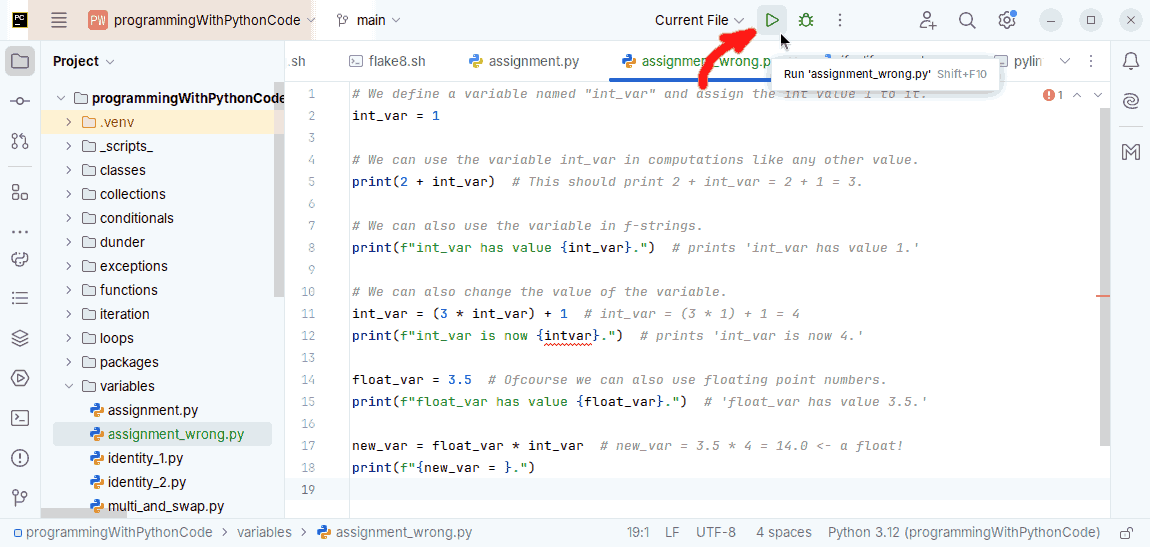
\includegraphics[width=0.9\linewidth]{\currentDir/errorsInIde01runProgram}}}%
%
\floatRowSep%
%
\subfloat[][%
The output in the run window is the same as given in \cref{exec:variables:assignment_wrong}. %
It is the \emph{first} way to find out what went wrong. %
It tells us what went wrong and even suggests how to fix it:~\emph{\pythonilIdx{NameError}: name \inSQuotes{\pythonil{intvar}} is not defined. Did you mean: \inSQuotes{\pythonil{int_var}}?} %
It also tells us the exact file and line where the error occurred, namely in line~12 of file \textil{assignment_wrong.py}.%
\label{fig:errorsInIde02exception}%
]{\tightbox{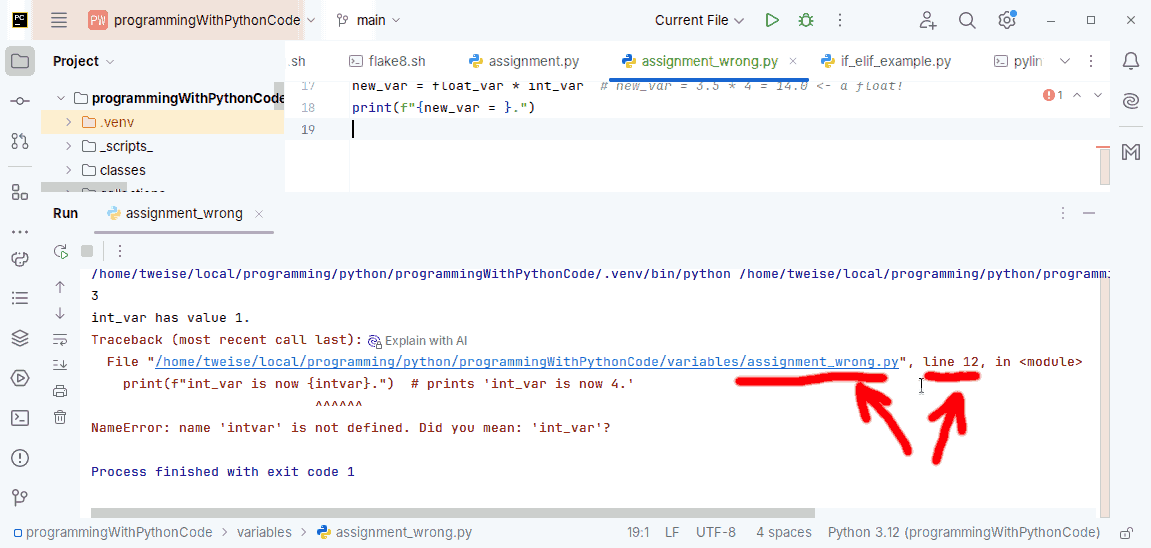
\includegraphics[width=0.9\linewidth]{\currentDir/errorsInIde02exception}}}%
%
\floatRowSep%
%
\subfloat[][%
If we click on the linked file location, it takes us to where the error occurred. %
The incorrectly typed word is (and always was) underlined with red color. %
Looking for underlined words is the \emph{second} method to find errors in code!%
This should have told us already that something is fishy without the need to even run the program in the first place.%
\label{fig:errorsInIde03underlined}%
]{\tightbox{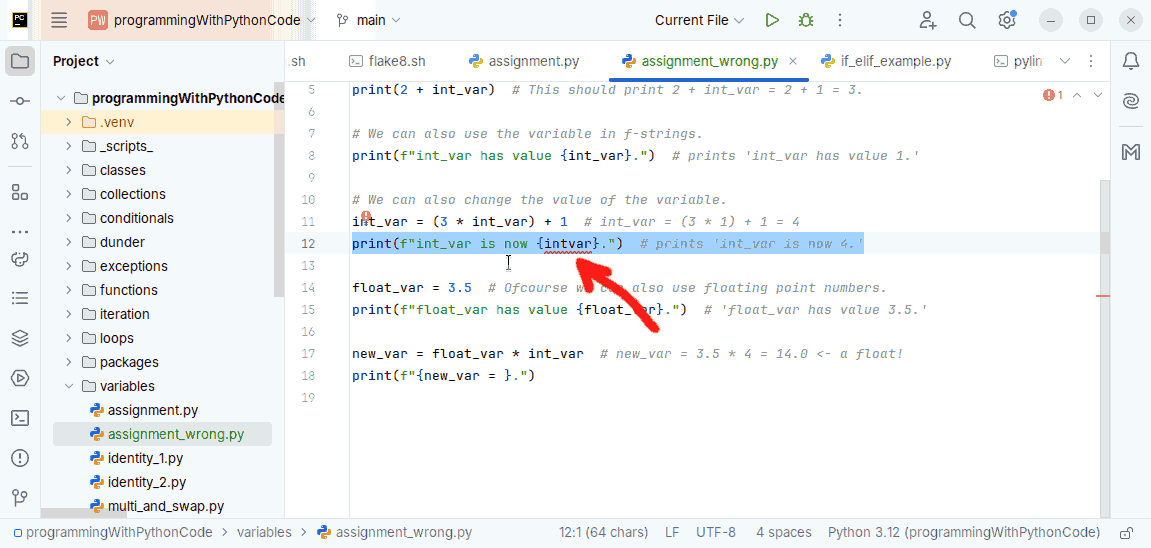
\includegraphics[width=0.9\linewidth]{\currentDir/errorsInIde03underlined}}}%
%
\caption{How the \pgls{ide} can help us finding errors.}%
\label{fig:errorsInIdeA}%
\end{figure}%
%
\begin{figure}%
\ContinuedFloat%
\centering%
%
\subfloat[][%
The \pgls{ide} also informs us that something is wrong by displaying the small red~\pycharmErrorsSymbol~icon in the top-right corner. %
This is the \emph{third} way to find errors. %
We click on it\dots%
\label{fig:errorsInIde04errors}%
]{\tightbox{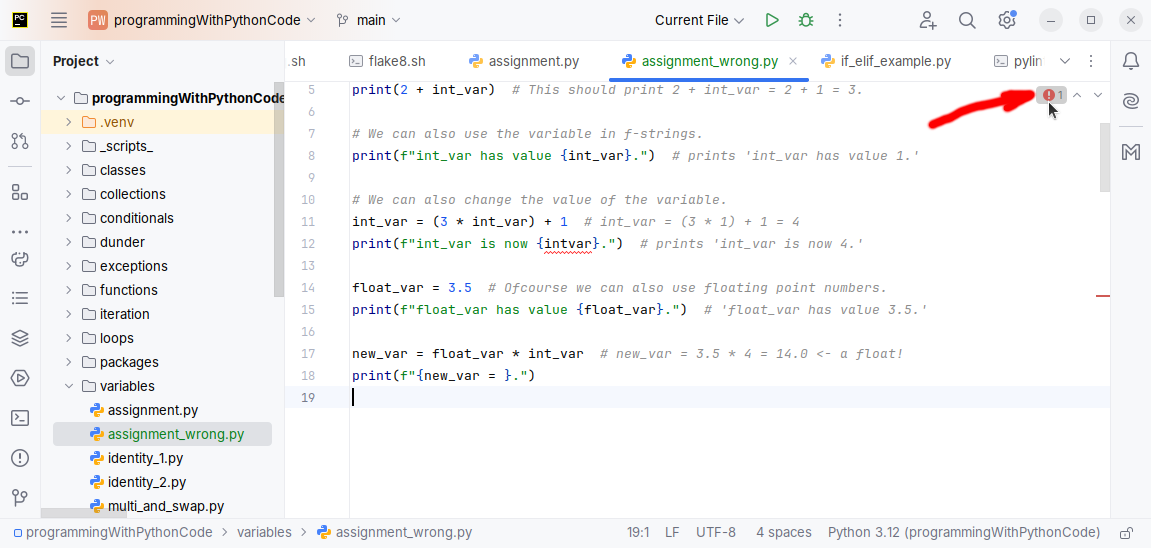
\includegraphics[width=0.9\linewidth]{\currentDir/errorsInIde04errors}}}%
%
\floatRowSep%
%
\subfloat[][%
{\dots}and it takes us to the list of potential errors that it has detected. %
Here, it tells us that there is an \emph{Unresolved reference \inSQuotes{intvar}} at line~12 of the file. %
We click on this note\dots%
\label{fig:errorsInIde05errorsList}%
]{\tightbox{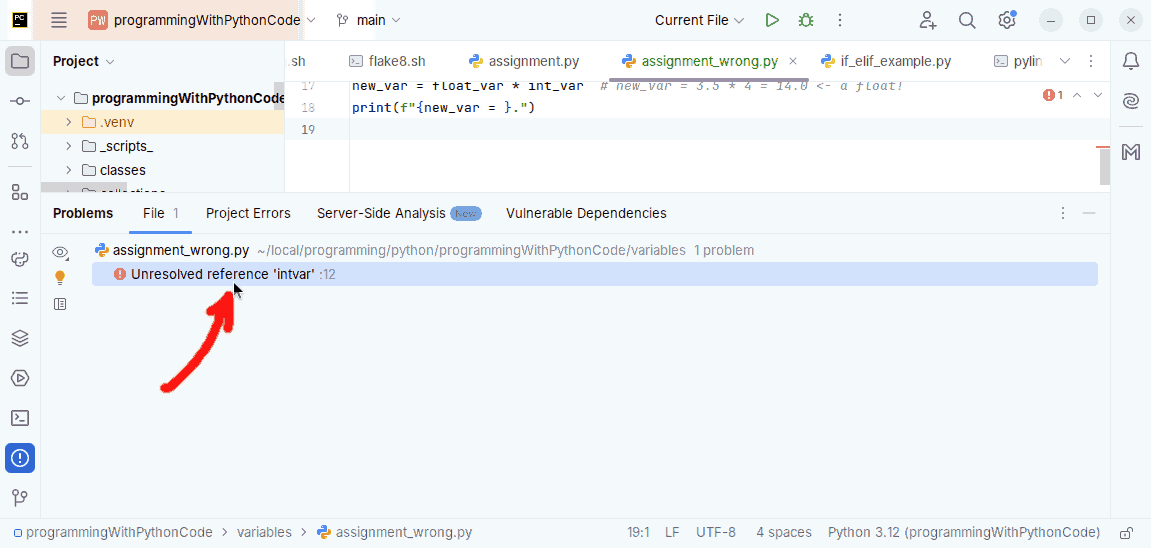
\includegraphics[width=0.9\linewidth]{\currentDir/errorsInIde05errorsList}}}%
%
%
\floatRowSep%
%
\subfloat[][%
{\dots}and it takes us again to the dodgy line.%
\label{fig:errorsInIde06errorsListToLine}%
]{\tightbox{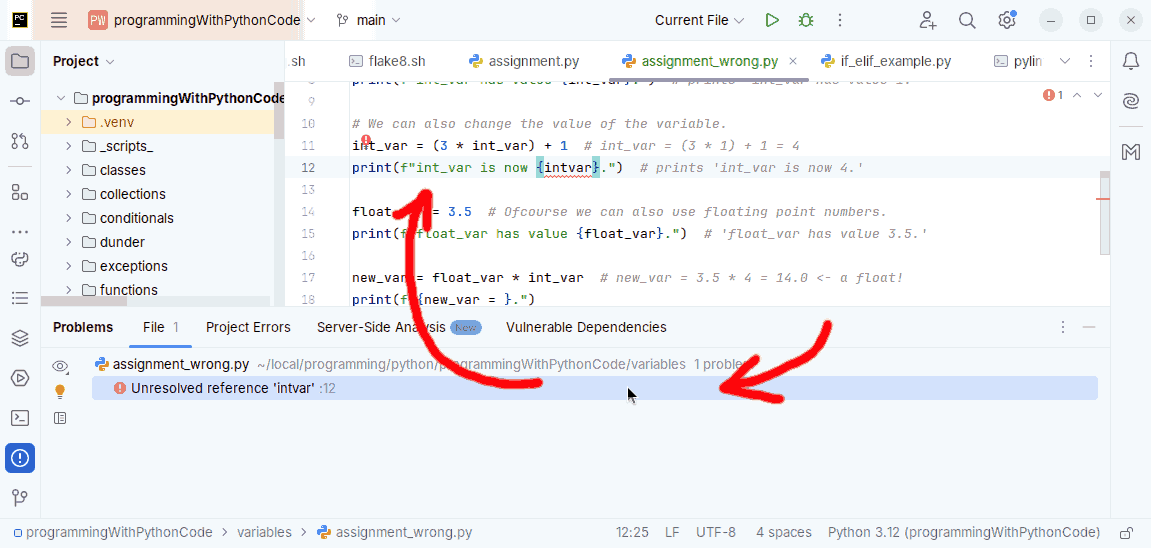
\includegraphics[width=0.9\linewidth]{\currentDir/errorsInIde06errorsListToLine}}}%
%
\caption{How the \pgls{ide} can help us finding errors.}%
\label{fig:errorsInIdeB}%
\end{figure}%
%
\begin{figure}%
\ContinuedFloat%
\centering%
%
\subfloat[][%
The \emph{fourth} way in which the \pycharm\ \pgls{ide} can help us to discover errors are small red marks at the right-hand side. %
Holding the mouse cursor over these lines will open a small view with the suggested error message.%
\label{fig:errorsInIde07errorMark}%
]{\tightbox{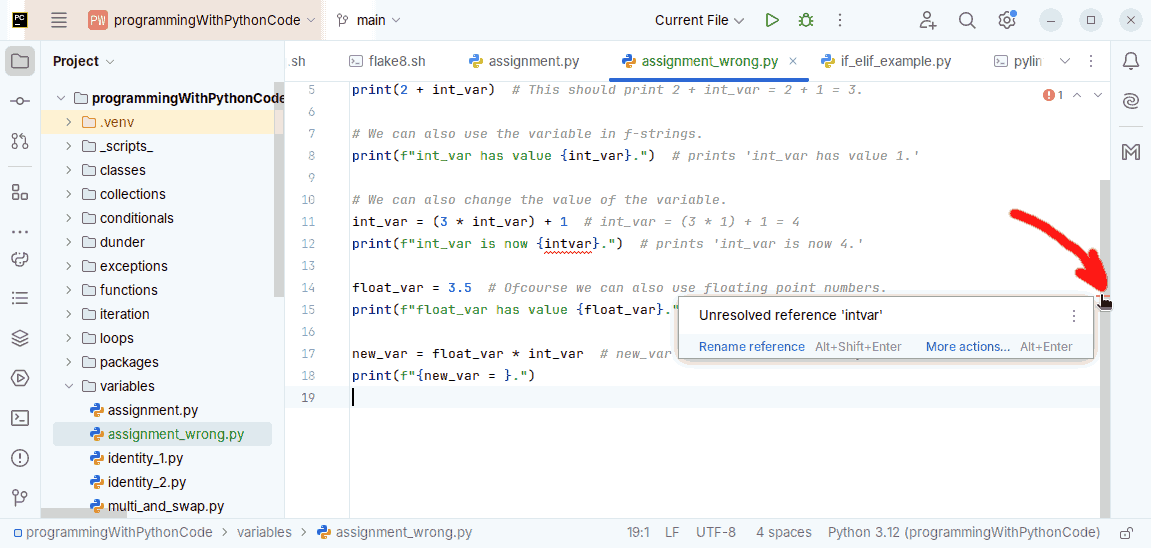
\includegraphics[width=0.9\linewidth]{\currentDir/errorsInIde07errorMark}}}%
%
\floatRowSep%
%
\subfloat[][%
The \emph{fifth} way to get a list of potential errors in \pycharm\ is to click on the \pycharmErrorsButton~button in the side menu on the left-hand side or to press~\keys{\Alt+6}.
\label{fig:errorsInIde08sidebar}%
]{\tightbox{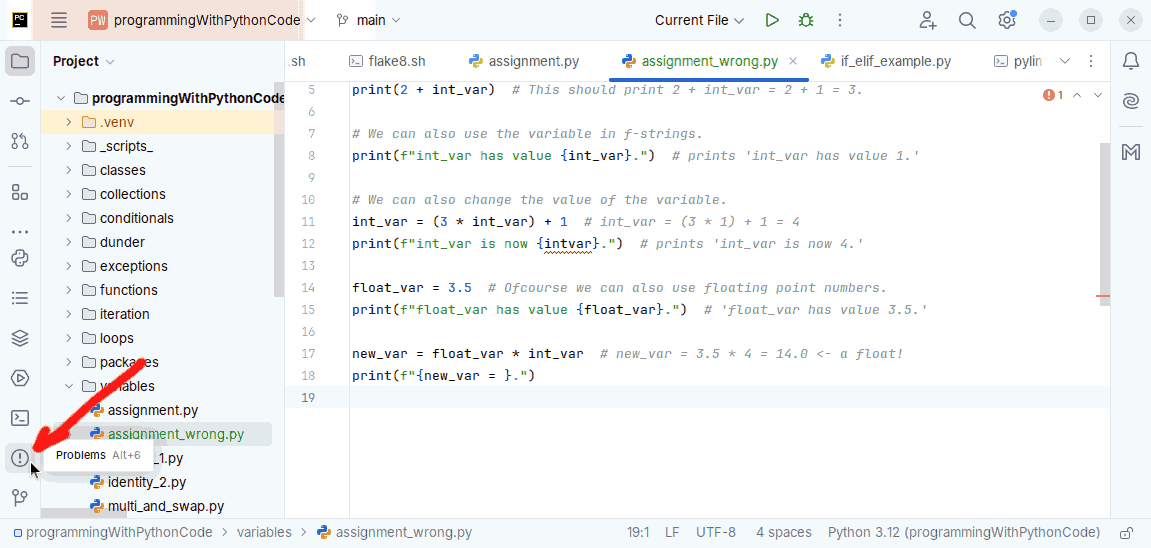
\includegraphics[width=0.9\linewidth]{\currentDir/errorsInIde08sidebar}}}%
%
\floatRowSep%
%
\subfloat[][%
This again takes us to the list of potential errors.%
\label{fig:errorsInIde09sidebarToView}%
]{\tightbox{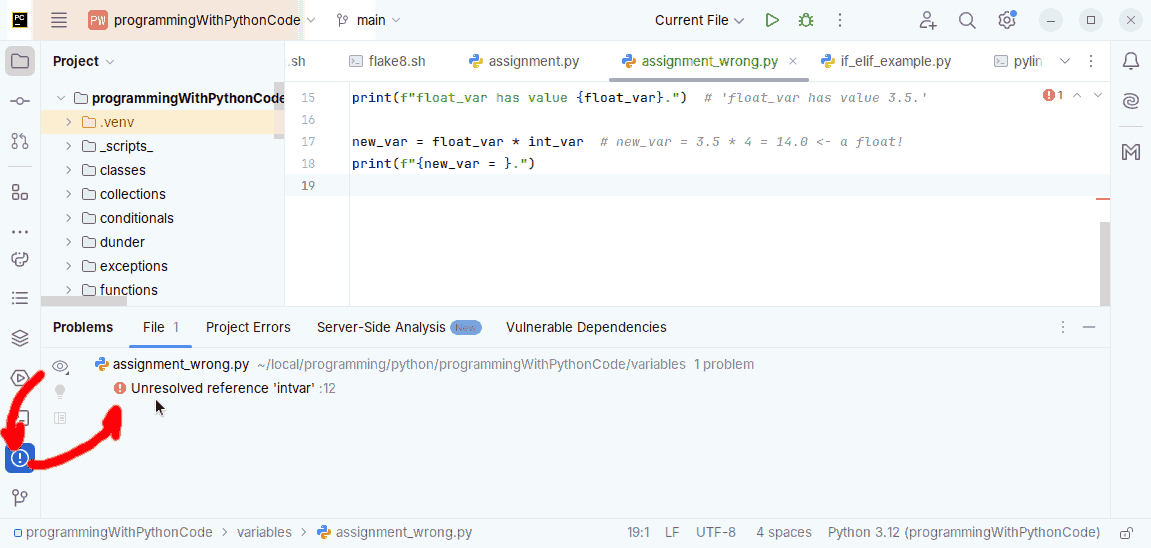
\includegraphics[width=0.9\linewidth]{\currentDir/errorsInIde09sidebarToView}}}%
%
\caption{How the \pgls{ide} can help us finding errors.}%
\label{fig:errorsInIdeC}%
\end{figure}%
%
Before we depart from \pycharm\ screenshots, however, we will visit one absolutely crucial functionality that modern \pglspl{ide} provide:
They help us to find errors in the code.
Errors are common.
They happen all the time.
All programmers make mistakes.
Sometimes it's a typo.
Sometimes we accidentally switch the order of parameters of a function.
Sometimes we mix up \pythonils{float} and \pythonils{int}.
Sometimes we make logical errors.
Sometimes we misunderstood what the function that we are calling does.
Sometimes we misunderstood the algorithm that we try to implement.
Some errors are obvious and easy to fix.
Some errors can be discovered based on the error output of the program.
Some errors require more serious \glslink{debugger}{debugging} to even spot them~(see \cref{sec:dunder:debugging}).
In some simple cases like typos, however, our \pgls{ide} can already point us to the mistake.%
%
%
\hsection{Finding the Error by using the Program Output and Exceptions}%
In \cref{lst:variables:assignment_wrong}, we prepared program \textil{assignment_wrong.py}, a variant of \textil{assignment.py}~(\cref{lst:variables:assignment}) with an error.
For the sake of the example, let us assume that the programmer made a typo in line~12 of the program:
They misspelled \pythonil{int_var} as \pythonil{intvar}.
Executing the program with the error leads to the output given in \cref{exec:variables:assignment_wrong}.

We can also open the program \textil{assignment_wrong.py} given in the \pycharm\ \pgls{ide}.
We execute this program manually by clicking on the \pycharmRun\ button or by pressing~\keys{\shift+F10} in \cref{fig:errorsInIde01runProgram}.
As you can see, the output in the run window is the same as given in \cref{exec:variables:assignment_wrong}~(\cref{fig:errorsInIde02exception}).

If a program crashes, then \emph{carefully} reading its output is always the \emph{first} way to find out what went wrong.
Indeed, in our example, the text that appeared tells us what went wrong and even suggests how to fix it.
It says:~\emph{\inQuotes{\pythonilIdx{NameError}: name \inSQuotes{\pythonil{intvar}} is not defined. Did you mean: \inSQuotes{\pythonil{int_var}}?}}
This is already pretty clear.
We accessed some variable~(a name), \pythonil{intvar}, which has not been defined or assigned.
It simply does not exist.

The \python\ interpreter then checks whether some similar name exists.
It found that there is a variable named \pythonil{int_var}.
Even more, it also tells us the exact file and line where the error occurred, namely in line~12 of file \textil{assignment_wrong.py}!
With this information, we have a good chance of finding the mistake.

The so-called \pythonilIdx{Exception} \pgls{stackTrace} that it prints to \pgls{stderr} thus not just tells us that there was an error.
It even tells us a probable cause and the most-likely line of code that caused the error.
We will discuss this topic in-depth later in \cref{sec:exceptions}, but even at this stage, the message here is pretty clear.%
%
\bestPractice{readErrorMessage}{Always carefully \emph{read} error messages. %
They often provide you very crucial information where to look for the mistake. %
Not reading error messages is wrong.%
}%
%
\endhsection%
%
\hsection{Finding the Error by using the IDE}%
%
We found the error by executing the program, seeing that it crashed, and then reading the output.
In the run console of \pycharm\ that presents the program output, we can even click on the linked file location.
This takes us to where the error occurred in \cref{fig:errorsInIde03underlined}.

The question is:
Could we have found this error even without executing the program?
Actually, when looking at the line to which the click took us, we notice that the incorrectly typed word is~(and always was) underline with red color.
This should have told us already that something is fishy without the need to even run the program in the first place.%
%
\bestPractice{redUnderline}{%
When writing code, we should always check whether the \pgls{ide} notifies us about potential errors. %
In the case of \pycharm, these are often underlined in red or yellow color. %
We should always check all such marks!%
}%
%
So we already know two ways in which we can find errors in our code with the help of our \pgls{ide}.
But there are even more ways.

The \pgls{ide} also informs us that something is wrong by displaying the small red~\pycharmErrorsSymbol~icon in the top-right corner, as shown in \cref{fig:errorsInIde04errors}.
Clicking on this symbol is the third way to find errors.
This will take us to the list of potential errors that it has detected in \cref{fig:errorsInIde05errorsList}.
Here, \pycharm\ tells us that there is an \emph{\inQuotes{Unresolved reference \inSQuotes{intvar}}} at line~12 of the file.
We can also click on that note, and  it takes us again to the dodgy line in \cref{fig:errorsInIde06errorsListToLine}

The fourth method in which the \pycharm\ \pgls{ide} can help us to discover errors are small red marks at the right-hand side of our editor window, shown in \cref{fig:errorsInIde07errorMark}.
Holding the mouse cursor over these marks will open a small view with the suggested error message.

The fifth way to get a list of potential errors in \pycharm\ is to click on the \pycharmErrorsButton~button in the side menu on the left-hand side or to press~\keys{\Alt+6}, as illustrated in \cref{fig:errorsInIde08sidebar}.
This again takes us to the list of potential errors in \cref{fig:errorsInIde09sidebarToView}.
%
\usefulTool{ideForErrors}{%
The \pgls{ide} and the error messages (\pythonilIdx{Exception} \pglspl{stackTrace}) are your most important tools to find errors. %
Read error messages. %
If your \pgls{ide}  -- regardless whether it is \pycharm\ or something else -- annotates your code with some marks, then you should check every single one of them.%
}%
\endhsection%
%
%
\hsection{Summary}%
Programmers make errors.
We make errors.
You are going to make lots of errors.
Later and now.
Even now, in very simple programs, we are going to make errors.
This cannot be prevented.
The question can only be how we deal with that.
How can we minimize the number of errors that we are going to make?
How can we maximize that chance to discover and fix errors?

The answer is simple:~\emph{By using all the tools at our disposal.}
We can use the output of programs to find errors after running the programs.
And we can use our \pgls{ide} to find errors based on the hints it provides to us even before executing the programs.
Both tools make it much much easier to find errors.
You can guess the importance of error-finding features also by the fact that \pycharm\ implements the error hints in several different ways, in the hope to get you to click and investigate its list of proposed errors and warnings.
As mentioned in \cref{bp:readErrorMessage,bp:redUnderline}, using the \pgls{ide} features for error discovery and detection is incredibly important.

Even if your program executes as expected, there still might be hidden errors in the code.
Sometimes, you can easily tell whether the output of a program is correct.
Sometimes, you cannot.
In some cases, an output that looks OK might still be wrong.

Sometimes, there might be some incorrect instructions in your program that just weren't used in your last execution.
So even correct program output does not guarantee that the program itself is correct.
Therefore, always checking each and every piece of code that your \pgls{ide} marks as dodgy is very important.
Make sure that you full understand all error and warning messages.

Warnings can be important, too.
They can indicate possible errors, potential problems with variable types, or missing required packages~(see, e.g., \cref{sec:gitClonePycharm}).
Always fix errors and warnings wherever possible~(obviously).
Even where you deem the warnings as false-positives, try to fix them anyway.
They could result from non-standard code formatting that still \inQuotes{works}, but may be confusing for readers of your code.
You should always try to produce warning-free code.
For every warning or error that you deem as not a problem, remember:
On one hand, \emph{you} might wrong.
On the other hand, having fewer warnings and false-positive suspected errors makes it easier to find the actual problem if an actual problem happens.%
%
\endhsection%
\FloatBarrier%
\endhsection%
%
